\chapter{Rappresentazione dei parcheggi sulla mappa}

Tutti i procedimenti descritti in precedenza, come la raccolta dei dati, le
operazioni che vengono effettuate su di essi, la predizione del tipo di 
parcheggio, ecc. portano al risultato di ottenere una serie di istanze
di parcheggio, all'interno del database, che possiedono varie informazioni.
Ogni parcheggio, tra le altre cose, può essere fornito di:
\begin{itemize}
    \item \textbf{coordinate finali}, che indicano il punto geografico dove l'auto ha 
    parcheggiato, sono sempre presenti (a volte potrebbero essere invalide)
    \item \textbf{tipo di parcheggio selezionato dall'utente}, presente per i parcheggi
    per cui è stata selezionata manualmente una etichietta di classificazione.
    \item \textbf{tipo di parcheggio predetto dal modello ML}, presente per i parcheggi
    per cui è stata effettuata la predizione con il modello (a meno di eccezioni, dovrebbe
    essere sempre presente)
    \item \textbf{valore di heading finale}, presente per i parcheggi
    per cui è stata effettuata la predizione con il modello (a meno di eccezioni, dovrebbe
    essere sempre presente)
\end{itemize}
Queste informazioni possono essere utilizzate per fornire dei benefici all'utente.
Di fatto, tutto il lavoro che porta a questo punto ha come scopo finale lo 
sfruttamento delle informazioni acquisite per arricchire l'esperienza 
dell'utente in qualche modo.\\
In particolare, l'obiettivo principale era l'ottenimento del tipo di parcheggio, ma 
attraverso l'intero procedimento è stato possibile ottenere anche il valore della 
bussola senza dover fare sforzi aggiuntivi.\\
I due utilizzi principali di queste informazioni, che vengono fatti per il momento, sono
mostrare visivamente sulla mappa i tipi di parcheggio alle rispettive coordinate, e
migliorare l'algoritmo di creazione dei match tra utenti che lasciano un parcheggio e 
quelli che ne cercano uno.\\
Mostrare i parcheggi sulla mappa offre all'utente la possibilità di poter trovare 
facilmente delle zone di posteggio in un'area a proprio piacimento. Integrare
nelle figure dei parcheggi anche altri dettagli, come il tipo di parcheggio o 
l'orientamento, può ulteriormente facilitare l'esperienza dell'utente, ad esempio
facendogli capire in anticipo com è fatto il parcheggio che sta cercando.
Ad ogni modo, la rappresentazione grafica che è stata implementata all'interno
dell'app GeneroCity si tratta di una versione non definitiva, quindi poco affinata e poco
testata sull' utente finale. Dato che l'app non è ancora stata rilasciata, questa 
rappresentazione è utilizzata principalmente per lo sviluppo ed è destinata a subire
grandi miglioramenti dal punto di vista grafico e dell'interfaccia. Nonostante ciò,
la logica che la gestisce e il proprio ciclo di vita, che viene giostrato dagli eventi
dell'interfaccia utente, sono sufficentemente maturi e pronti ad un potenziale rilascio.\\
Invece, per quanto riguarda l'algoritmo di matching, esso viene utilizzato per 
rendere possibile uno scambio di parcheggio tra un utente che sta lasciando lo 
stesso e un altro che ne sta cercando uno. Essendo a conoscenza dei tipi dei 
parcheggi, al momento della ricerca di un parcheggio disponibile da parte di un
utente che possa prendere il posto lasciato, si potranno preferire i posti in cui
è più probabile che l'auto di colui che cerca entri e scartare quelli in cui invece
probabilmente l'auto non entrerà a causa delle dimensioni.\\
Tuttavia, in sviluppi futuri, queste informazioni potranno essere sfruttate anche in
altri ambiti, o semplicemente per migliorare in altri modi i servizi già esistenti.


\section{Recupero dei parcheggi nella zona visualizzata} 

Mostrare una rappresentazione grafica dei parcheggi all'utente richiede, come prima cosa,
l'ottenimento delle informazioni necessarie su di essi. Per ogni \emph{Car} presente nel 
sistema, vengono salvati nel database tutti i parcheggi effettuati, costituiti dalle 
informazioni descritte in precedenza, ed altre, tra cui il timestamp del caricamento.\\
Occorre quindi un metodo per scaricare le informazioni riguardanti i parcheggi che 
devono essere rappresentati sulla mappa. In particolare, quando l'utente osserva una
specifica porzione della mappa, ha bisogno di vedere tutti i parcheggi che si trovano 
in quella determinata zona e nessun altro. Questo ha permesso una progettazione che 
minimizzasse la quantità di richieste inviate all'API backend e allo stesso tempo 
mostrasse visivamente tutti i parcheggi in maniera fluida e senza provocare
interruzioni all'esperienza utente. Chiaramente, l'area inquadrata nella mappa 
cambia molto frequentemente e a seconda di come l'utente interagisce con essa. 
Quindi, l'algoritmo di recupero dei parcheggi deve tenere conto anche di questo fatto
ed impedire che vengano invocate un numero eccessivo di chiamate verso il server.\\
Dunque, è stato necessario introdurre una nuova funzione fornita dall'API del backend
di GeneroCity, che permettesse di scaricare le istanze dei parcheggi in maniera
intelligente. Successivamente, è stato progettato un algoritmo che potesse sfruttare
al meglio la nuova funzione introdotta e quindi scaricare le informazioni sui parcheggi,
tenendo conto di tutti i vincoli presenti e le necessità dell'utente finale.

\subsection{Chiamata API per la richiesta dei parcheggi in un'area}

In GeneroCity iOS sono state utilizzate le mappe di Apple, che vengono distribuite
attraverso la libreria \emph{MapKit\footnote{MapKit page on Apple's website: 
\href{https://developer.apple.com/documentation/mapkit}{\underline{link to the page.}}}}
\cite{introduction_apple_maps_mapkit}.
La classe responsabile della rappresentazione
grafica di una mappa è \emph{MKMapView}. Quest'ultima possiede un attributo \textbf{region}
che corrisponde all'informazione sull'area mostrata sullo schermo nell'istante corrente.
Infatti, quando l'area visibile sul display cambia (ad esempio in seguito ad uno swipe
dell'utente), anche la \textbf{region} viene aggiornata. Questo oggetto è formato dalle
coordinate del centro dell'area interessata e da due valori che rappresentano lo 
scostamento di longitudine e quello di latitudine. Gli scostamenti indicano rispettivamente gli
angoli, espressi in gradi, tra la longitudine minore e quella maggiore e la latitudine 
minore e quella maggiore visibili attualmente sullo schermo. In questo modo, si è a conoscenza della porzione esatta di mappa visibile dall'utente
in ogni istante.\\
Si può utilizzare questa informazione per ottenere le istanze dei parcheggi che si trovano 
nel database e che sono stati registrati all'interno dell'area richiesta.
Dati i parametri \textbf{lat} (latitudine del centro dell'area), \textbf{lon} 
(longitudine del centro dell'area), \textbf{deltaLat} (scostamento di latitudine), 
\textbf{deltaLon} (scostamento di longitudine), l'interrogazione
al database consiste semplicemente nella selezione dei parcheggi \textbf{p}, relativi
a qualsiasi auto, tali che:
\begin{center}
    $ \textbf{lat} - \textbf{deltaLat} \le \textbf{p.latitude} \le \textbf{lat} + \textbf{deltaLat}$\\
    e\\
    $ \textbf{lon} - \textbf{deltaLon} \le \textbf{p.longitude} \le \textbf{lon} + \textbf{deltaLon}$
\end{center}
Questa interrogazione è stata inserita all'interno di una nuova chiamata API, di tipo "GET".
Questa chiamata è stata definita "Get area park list", in quanto restituisce la lista di 
parcheggi presenti all'interno dell'area indicata.\\
I parametri accettati dalla chiamata sono tutti e soli quelli appena definiti,
tutti di tipo float. Inoltre, tutti i parametri sono obbligatori, in quanto 
sono tutti essenziali per il corretto calcolo del risultato.\\
La risposta fornita da questa chiamata consiste in una lista di oggetti in formato JSON, 
contenenti le informazioni dei singoli parcheggi trovati. Ogni oggetto di un parcheggio
contiene: le coordinate, il timestamp, le etichette del tipo di parcheggio (sia quella 
selezionata dall'utente che quella predetta dal modello classificatore), l'heading, ecc.
Qualora nel database alcuni di questi campi non fossero obbligatori, i rispettivi valori 
restituiti potrebbero essere nulli.\\
All'interno del modulo API dell'app Generocity iOS è stata quindi aggiunta una una funzione
di interfaccia, in grado di effettuare una chiamata alla funzionalità backend appena descritta.
% TODO: maybe add a picture of the architecture for the call (frontend > backend > DB -<)
Tra i vari parametri della funzione è presente una callback, che viene eseguita nel momento in cui
viene ricevuta la risposta dal server. Questa callback contiene un oggetto JSON, che è esattamente
la lista delle istanze dei parcheggi trovati. In questo modo, è possibile ottenere la lista desiderata in maniera asincrona, direttamente con una chiamata a funzione. 

\subsection{Scheduling delle richieste}

Come è stato anticipato, i parcheggi che devono essere mostrati sulla mappa devono essere 
scaricati con un criterio che tenga conto di diversi vincoli. Al centro di tutto vi è
l'esperienza dell'utente. Infatti, si è cercato di progettare un algoritmo di recupero dei 
parcheggi che permettesse di mostrare immediatamente, o comunque con poco ritardo, le 
istanze sulla mappa. Inoltre, si è tentato di far mantenere questa proprietà anche in seguito
ad un potenziale cambiamento della regione di mappa visibile sullo schermo, causato da uno
swipe dell'utente stesso, o da qualsiasi evento all'interno dell'app. Questo può essere
classificato come un requisito funzionale. Di contro, possono essere individuati diversi
requisiti non funzionali che pongono dei vincoli e delle limitazioni che devono essere 
rispettati per garantire la fattibilità di questa funzionalità:
\begin{itemize}
    \item \textbf{richiesta della sola area visibile}: al crescere del numero di parcheggi 
    salvati nel database, aumenta la densità dei parcheggi in una data zona e quindi 
    aumenta il numero di potenziali istanze da scaricare. Al fine di contenere le 
    dimensioni del payload delle risposte ricevute dal server, conviene ridurre il più
    possibile la grandezza della zona richiesta, idealmente soltanto l'area circostante
    la \textbf{region} attualmente visibile. Questo meccanismo non sarà comunque 
    sufficiente per quando il numero dei parcheggi presenti nel database diverrà
    molto grande. Con sviluppi futuri dell'app si potrà risolvere il problema, ad 
    esempio richiedendo solo i parcheggi registrati in un certo intervallo di tempo,
    oppure ponendo un limite alla lunghezza della lista in risposta.
    \item \textbf{intervallo di tempo tra due richieste all'API}: la regione della mappa
    visualizzata sullo schermo può cambiare molte volte e molto rapidamente. Questo fatto
    potrebbe creare problemi se implicasse un invio non controllato di richieste. Infatti,
    dato che l'evento di cambiamento della \textbf{region} della mappa viene lanciato per 
    ogni piccola variazione, l'effettuare una nuova richiesta ogni volta potrebbe 
    generare decine di chiamate al secondo. Questa cosa sarebbe chiaramente inutile e 
    deleteria, perché il server verrebbe inondato di richieste che oltretutto 
    richiederebbero una lista quasi uguale di parcheggi. Anche nel lato client questo 
    sarebbe dannoso, dovendo gestire un traffico troppo elevato di richieste e risposte
    HTTP. Viene naturale pensare quindi che sia necessario un limite sul numero di 
    richieste effettuabili in un certo intervallo di tempo.
    \item \textbf{richieste di aree molto grandi}: la mappa offre la possibilità di 
    modificare lo zoom della visuale, così da ingrandire e rimpicciolire l'area 
    visibile sullo schermo. Quando viene applicato uno zoom molto basso e quindi 
    l'area visibile si ingrandisce in maniera considerevole, le zone di posteggio
    diventano troppo piccole e invisibili all'utente. Questo significa che quando
    la \textbf{region} della mappa è molto grande, non ha senso mostrare la 
    rappresentazione dei parcheggi. Inoltre, richiedere la lista dei parcheggi
    registrati in una grande zona porterebbe al problema già discusso di una
    quantità di istanze trovate troppo grande. Questo farebbe sorgere dei 
    problemi relativi anche alla quantità elevata di memoria occupata nel
    sistema operativo per l'applicazione.
    \item \textbf{richieste della stessa area}: quando la \textbf{region} della mappa
    cambia di un piccolo delta, la maggior parte dei parcheggi richiesti sarebbero
    gli stessi che erano stati ottenuti alla richiesta precedente. Quindi, si possono
    evitare richieste duplicate per la stessa zona e occorre un metodo per evitare 
    di inviare richieste inutili.
\end{itemize}
Con lo scopo di soddisfare tutti questi requisiti, è stato progettato un algoritmo di 
scaricamento dei parcheggi che effettua diversi controlli prima di procedere con una 
nuova richiesta. \'E stata così definita una classe \emph{ParkingOverlaysLoader}, 
responsabile dell'esecuzione delle richieste all'API. Un'istanza di questa classe
viene gestita dalla mappa. In particolare, vengono sfruttati degli eventi generati
dalla mappa per chiamare il metodo \emph{load()} di \emph{ParkingOverlaysLoader} e
quindi effettuare una nuova richiesta, se questa viene permessa.\\
Come già annunciato, la mappa genera un evento ogni volta che la \textbf{region} è 
soggetta ad un piccolo cambiamento. Questo evento può essere catturato attraverso
il metodo \emph{mapViewDidChangeVisibleRegion()}, offerto dal delegate della mappa
stessa. In questo modo, si può effettuare una chiamata al metodo \emph{load()} e
lasciar gestire al \emph{ParkingOverlaysLoader} la scelta di compiere o no una
nuova richiesta.\\
Dopo la prima chiamata, che genera sempre una richiesta all'API, entreranno in regime
una serie di condizioni che ogni volta controlleranno se sia il caso di procedere con
una nuova richiesta. Sono utilizzate delle variabili che mantengono lo stato del 
\emph{ParkingOverlaysLoader}: \textbf{lastQueryTimestamp} in cui viene salvato 
l'istante dell'ultima richiesta e \textbf{lastQueryRegion} in cui viene invece 
ricordata l'area per cui è stata fatta l'ultima richiesta. Definendo 
\textbf{MIN\_TIME\_BETWEEN\_QUERIES} come il tempo minimo
che deve passare tra una richiesta e la successiva e \textbf{MAX\_REGION\_DELTA} come 
il massimo scostamento (angolo in gradi) tra i due estremi visibili della mappa per 
cui abbia senso effettuare una richiesta, vengono controllate le seguenti condizioni:
\begin{center}
    $ \textbf{mapView.region.span.latitudeDelta} > \textbf{MAX\_REGION\_DELTA} $
\end{center}
controlla che la visuale attuale abbia una \textbf{region} più grande della massima
permessa. Quindi il numero dei potenziali parcheggi presenti sarebbe troppo elevato.
\begin{center}
    $ \textbf{Date().timeIntervalSince1970} - \textbf{self.lastQueryTimestamp} < 
    \textbf{MIN\_TIME\_BETWEEN\_QUERIES} $
\end{center} 
controlla che il tempo trascorso dall'ultima richiesta al momento attuale sia minore 
del limite minimo predisposto. In questo caso si invierebbe una richiesta dopo troppo
poco tempo rispetto alla precedente.
\begin{center}
    $ abs(\textbf{mapView.region.center.latitude} - \textbf{lastQueryRegion.center.latitude}) < \textbf{lastQueryRegion.span.latitudeDelta}/2 $\\
    e\\
    $ abs(\textbf{mapView.region.center.longitude} - \textbf{lastQueryRegion.center.longitude}) < \textbf{lastQueryRegion.span.longitudeDelta}/2 $\\
    e\\
    $ \textbf{mapView.region.span.latitudeDelta} < \textbf{lastQueryRegion.span.latitudeDelta} * 1.5) $
\end{center} 
controlla che la zona attualmente visualizzata sulla mappa non sia cambiata abbastanza
rispetto a quella dell'ultima richiesta. Come descritto più avanti, la richiesta
viene effettuata per una zona leggermente più grande di quella visibile, e così, 
quando la visuale si muove di un piccolo delta, i parcheggi caricati in precedenza
riescono ancora a coprire l'intera area visibile. In questo caso, non è necessario
scaricare i parcheggi nuovamente. Da notare che la zona inquadrata sulla mappa può
variare anche venendo rimpicciolita o ingrandita, e non solo venendo traslata. Quindi,
può accadere che l'utente rimpicciolisca la mappa e quindi esca fuori dalla zona coperta
dall'ultimo scaricamento. La terza condizione in "and" logico controlla che questo
non accada.\\

Se almeno una di queste macro-condizioni è soddisfatta, la richiesta all'API viene 
interrotta, altrimenti vengono aggiornate le variabili con i dati attuali e si prosegue.\\
Quindi viene effettivamente chiamata la funzione collegata all'API (definita in precedenza)
e inviata la richiesta. I parametri \textbf{deltaLat} e \textbf{deltaLon} vengono presi 
il doppio dello scostamento che dal centro della mappa va fino al bordo della porzione
di area visibile. In questo modo, il server risponderà con una lista di parcheggi che 
include anche le istanze che si trovano nelle estreme vicinanze dell'area visibile.

\section{Disegno dei parcheggi sulla mappa} 

Una volta che è stata definita la dinamica per lo scaricamento delle istanze di 
parcheggio, c'è bisogno di un modo per salvare queste in locale e successivamente 
mostrarle visivamente sulla mappa.\\
Per impedire che lo scaricamento dei parcheggi vada a occupare troppa memoria 
all'interno dell'app, si è deciso di eliminare le istanze scaricate con una 
richiesta precedente, non appena arrivi il risultato di una nuova. Inoltre, 
così facendo, non si va ad applicare caching a particolari zone della mappa
e così, nel caso in cui vengano registrati nuovi parcheggi nel database, questi 
verranno scaricati non appena l'utente visualizzerà la zona interessata.\\
La maniera che fornisce \emph{MapKit} di disegnare delle forme sulla mappa è 
attraverso gli \emph{MKOverlay} \cite{displaying_objects_map}. Infatti, 
attraverso questi oggetti, è possibile
rappresentare forme di svariate tipologie, applicando colori, trasparenze e altro.
La lista degli overlay viene salvata come attributo della mappa e così 
è utilizzata per renderizzare tutte le forme sullo schermo, quando è necessario.\\
Per distinguere gli overlay relativi ai parcheggi da tutti gli altri, gli 
viene impostato il titolo a "parking", in modo da poter effettuare alcune operazioni 
esclusivamente su di essi. Ogni volta che viene ricevuta una nuova risposta dall'API, 
vengono eliminati tutti gli overlay dei parcheggi e poi ne vengono creati 
di nuovi, partendo dalle informazioni ricevute dal server. In particolare, viene 
impostato il centro dell'overlay alle coordinate del rispettivo parcheggio.\\
Dato che esistono overlay di forme diverse e personalizzabili, si è pensato di 
sfruttarli per rappresentare diverse informazioni riguardanti i parcheggi.

\subsection{Informazione sul tipo di parcheggio} 

Oltre alla presenza stessa di un parcheggio in un determinato punto, l'informazione
principale che si vuole rappresentare è quella del tipo del parcheggio stesso.
Per questo, al momento della creazione dell'overlay vengono salvate in esso 
entrambe le etichette del tipo selezionato dall'utente e di quello predetto
dal modello ML.\\
Sono state predisposte due diverse modalità di visualizzazione, sfruttando le 
forme del cerchio e del rettangolo. La prima è utilizzata per mostrare la 
presenza di un certa zona di parcheggio e il proprio tipo, mentre la seconda
rappresenta anche l'orientamento delle singole istanze, rispetto al nord geografico.\\
In forma non definitiva, è stato associato un colore primario ad ogni tipo di 
parcheggio e quindi questo verrà visualizzato dall'utente sulla mappa 
(Figura~\ref{fig:circle_overlays}). Inoltre,
si fa uso di un'alto livello di trasparenza in ogni overlay, in modo da far 
rafforzare la presenza di un colore, rispetto ad un altro, all'aumentare delle
istanze di parcheggio che coinvolgono le stesse coordinate (o coordinate molto
vicine). Così facendo, la presenza di un colore forte implica una grande 
accuratezza per un certo tipo di parcheggio (essendoci molte istanze dello stesso
tipo che si sovrappongono). Inoltre, le istanze di parcheggio molto vicine le une alle
altre vanno a colorare una intera zona in maniera abbastanza omogenea, e così mostrano
la presenza di un'intera area di posteggio.\\
% TODO: add screenshot with circles
Tuttavia, questo modo di rappresentare 
l'informazione non è risultato molto intuitivo per l'utente e quindi sarà utilizzato 
a scopo di sviluppo, mentre per il rilascio effettivo dell'applicazione verrà predisposta
una rappresentazione differente.

\subsection{Informazione sull'orientamento del parcheggio} 

Per quanto riguarda l'informazione sull'orientamento, si è pensato di riprodurre 
sulla mappa una forma simile a quella del rettangolo del parcheggio vero e 
proprio. Ovvero, si è provato a posizionare un overlay rettangolare alle coordinate
del parcheggio, orientato rispetto all'angolo ottenuto dal valore dell'heading
(Figura~\ref{fig:polygon_overlays}). 
\'E stato utilizzato un overlay poligonale, aggiungendo manualmente le coordinate
relative agli angoli del rettangolo. Inizialmente sono stati definiti due coefficienti 
di scostamento \textbf{ALPHA} e \textbf{BETA} per la formazione del rettangolo orientato 
verso il nord geografico. Così è stata creata la lista \textbf{points} di coordinate degli
angoli del rettangolo, relative all'origine. 
\begin{center}
    $ \textbf{points} = [[\textbf{BETA}, \textbf{ALPHA}],$\\
        $[\textbf{BETA}, -\textbf{ALPHA}],$\\
        $[-\textbf{BETA}, -\textbf{ALPHA}],$\\
        $[-\textbf{BETA}, \textbf{ALPHA}]] $
\end{center}
Successivamente, sono state moltiplicate le coordinate di base per la matrice \textbf{M} 
di rotazione 2D, in modo da ruotare il rettangolo iniziale ed ottenere 
l'orientamento desiderato. L'angolo $\theta$ di rotazione corrisponde al valore dell'heading, al negativo (la 
rotazione deve essere applicata nel senso opposto), convertito in radianti. 
\begin{center}
    $\textbf{M} = \begin{bmatrix}
        \cos{\theta} & -\sin{\theta}\\
        \sin{\theta} & cos{\theta}
    \end{bmatrix}$
\end{center}
Infine è stato applicata una traslazione, date le coordinate del parcheggio.
\begin{center}
    $CLLocationCoordinate2D($\\
    $latitude: \textbf{center.latitude} + $ \\
    $(\textbf{point}[0] * sin(\textbf{angle})) + (\textbf{point}[1] * cos(\textbf{angle})),$\\
    $longitude: \textbf{center.longitude} + $ \\
    $(\textbf{point}[0] * cos(\textbf{angle})) - (\textbf{point}[1] * sin(\textbf{angle})))$
\end{center}
% TODO: add screenshot with rectangles
Questa funzione si trova in stadio sperimentale, in quanto l'accuratezza del valore
dell'heading non è abbastanza elevata per rappresentare un orientamento realistico, 
bensì in diversi casi può accadere che il parcheggio venga orientato diversamente 
da come è in realtà. Inoltre, in questo caso, non è possibile sovrapporre diversi
parcheggi, perchè altrimenti si genererebbero delle forme prive di senso. In uno 
sviluppo futuro, si potrebbero fare più controlli sul salvataggio di parcheggi nel
database, magari cercando di capire quali istanze appartengono allo stesso posteggio
reale e quindi anche ottenere dati più accurati, combinando quelli provenienti da 
diverse istanze di uno stesso parcheggio.

\subsection{Rendering dei parcheggi}

Quando degli overlay vengono aggiunti alla mappa, questi sono pronti per essere
renderizzati sullo schermo, ma è necessario che vengano specificate delle informazioni
per impostare le proprietà grafiche delle varie tipologie. Per fare questo, il delegate
della mappa offre un metodo che viene chiamato appena prima che avvenga il rendering
di un overlay \cite{dynamic_rendering_map_information}. Tra i parametri vi è 
l'\emph{MKOverlay} stesso e il tipo di ritorno
è \emph{MKOverlayRenderer}, ovvero l'oggetto utilizzato dalla mappa per effettuare 
il rendering. All'interno di questo metodo vengono fatti i controlli per la selezione
della forma e dei colori dell'overlay. Infatti, come prima cosa si controlla il titolo
dell'overlay e se è uguale a "parking", si procede con le seguenti operazioni. Avviene
la differenziazione tra l'uso del \emph{MKCircle} e quello del \emph{MKPolygon}, per 
rappresentare il cerchio o il rettangolo del parcheggio. Infine, viene impostato
il colore dell'overlay in base al tipo di parcheggio specificato in esso.\\
Per permettere all'utente di disattivare la visualizzazione delle figure dei parcheggi
sulla mappa, è stata aggiunta una impostazione che viene modificata grazie ad uno switch.
Quando lo switch viene disattivato, tutti gli overlay dei parcheggi vengono eliminati 
dalla mappa e vengono interrotte le richieste all'API. Dato che la mappa si aggiorna 
automaticamente quando degli overlay vengono aggiunti o rimossi, tutte le figure 
dei parcheggi spariscono dallo schermo. Quando invece lo switch viene riattivato,
viene forzata una nuova richiesta all'API e vengono renderizzati nuovamente i parcheggi
presenti nella porzione di mappa visualizzata.

\begin{figure}
    \centering
    \begin{minipage}{.4\textwidth}
        \centering
        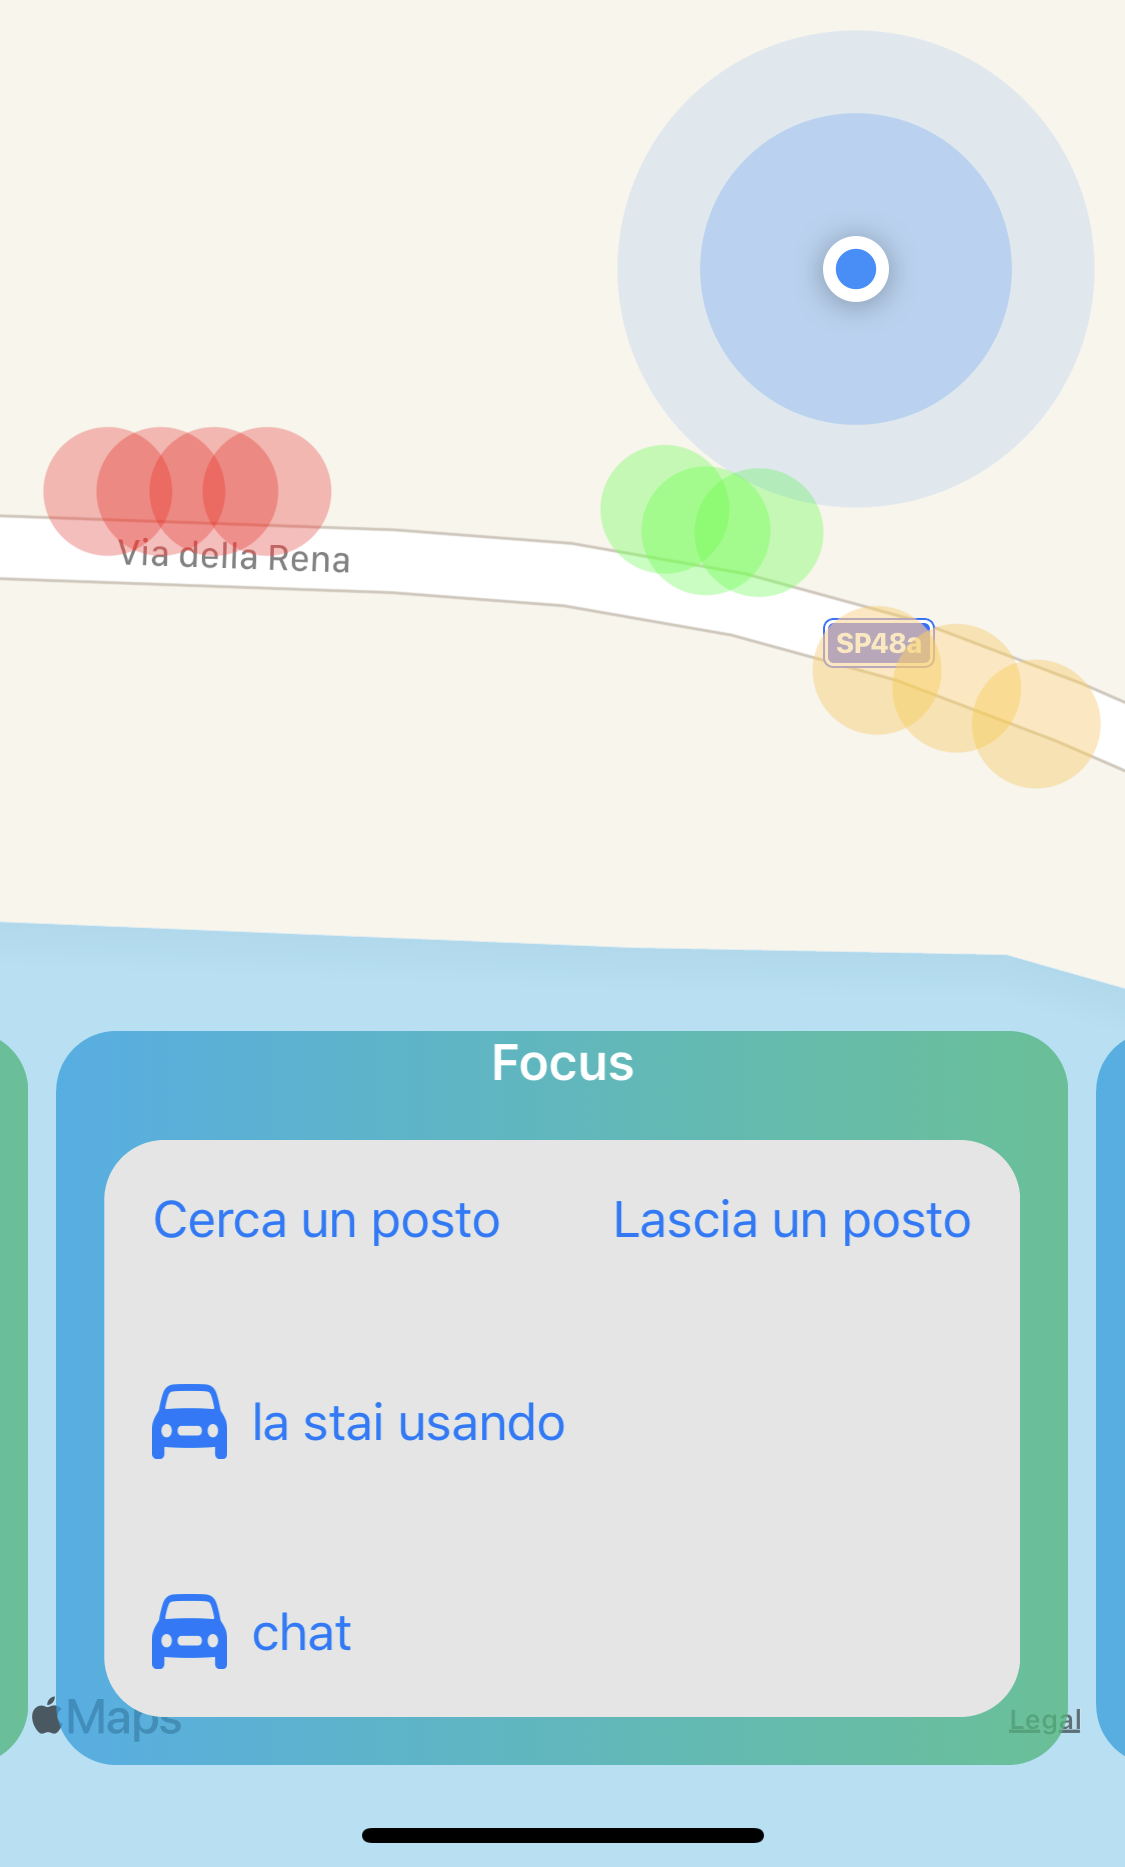
\includegraphics[width=5cm]{images/circle_overlays.png}
        \captionof{figure}{Mappa con la presenza di overlay di parcheggi circolari
        (giallo: parallelo, verde: a pettine, rosso: a spina).}
        \label{fig:circle_overlays}
    \end{minipage}
    \begin{minipage}{.4\textwidth}
        \centering
        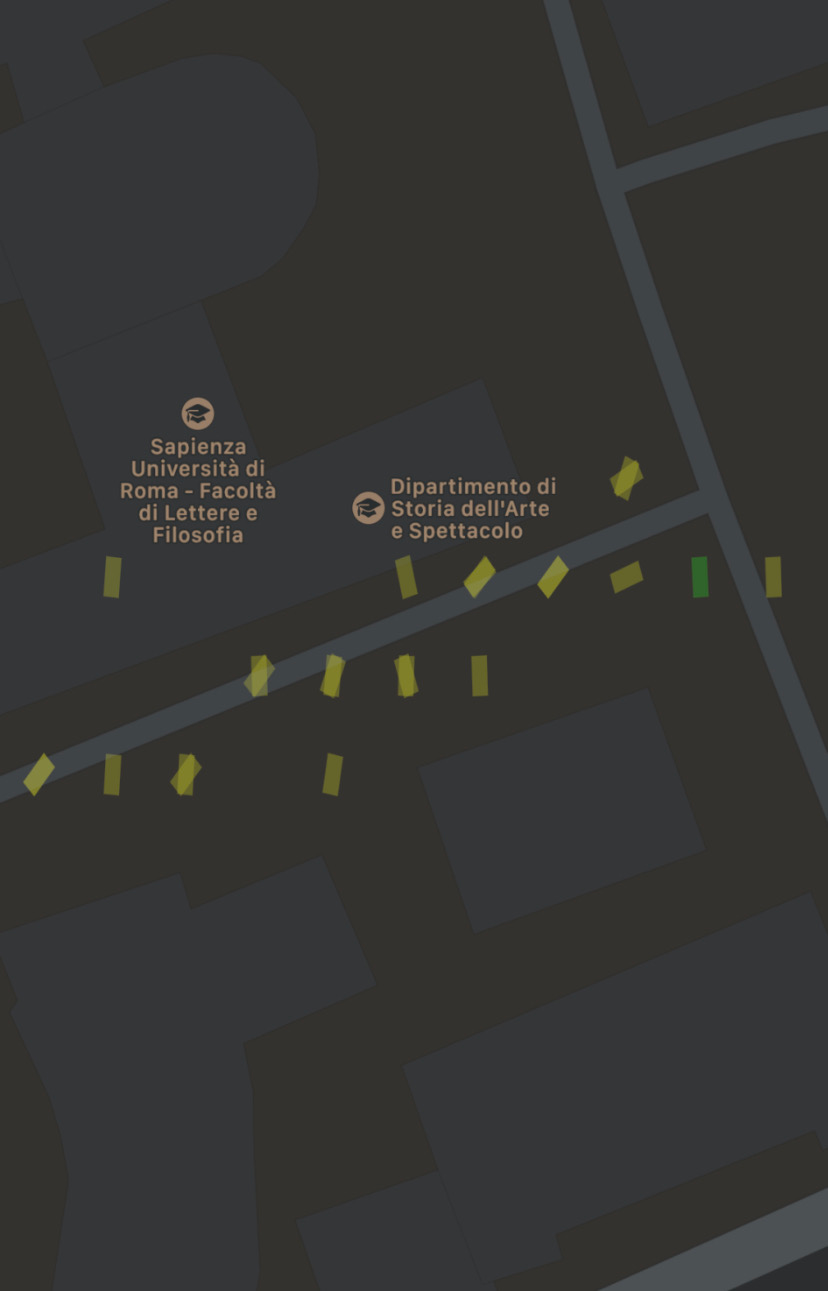
\includegraphics[width=5cm]{images/polygon_overlays.png}
        \captionof{figure}{Mappa con la presenza di overlay di parcheggi poligonali
        (giallo: parallelo, verde: a pettine, rosso: a spina).}
        \label{fig:polygon_overlays}
    \end{minipage}
\end{figure}


\section{Approccio crowdsource}

Come già discusso, l'approccio utilizzato per l'ottenimento delle istanze di parcheggio
fa leva sull'interazione implicita \cite{explicating_implicit_interaction}. Tutti i 
parcheggi caricati nel database
provengono da manovre di parcheggio reali e non sono stati inseriti manualmente dagli
sviluppatori. In questo modo, tenendo conto dei dovuti controlli di autenticità che 
dovranno essere applicati, si andranno a popolare di parcheggi tutte le zone in cui 
viene utilizzata l'app \cite{crowdsourcing_geospatial_data}. Di conseguenza, diventerà 
sempre più accurata l'informazione
sulla presenza di una determinata zona di posteggio in una specifica area. Questo 
approccio è quindi di natura molto scalabile e può essere sfruttato, con le dovute
accortezze, per facilitare un graduale incremento di utenza in diverse città e 
località.

\section{Beneficio dell'utente} 

L'intero lavoro portato avanti ha il fine di fornire dei benefici all'utente.
L'informazione riguardante il tipo di parcheggio può essere sfruttata in
diversi modi e averla a portata di mano potrebbe permettere in futuro di 
creare nuove funzionalità per cui essa risulti necessaria. Al momento della
scrittura sono stati individuati due casi d'uso principali per il dato: la 
rappresentazione visuale dei parcheggi (già descritta) e l'utilizzo all'interno 
dell'algoritmo di matching di utenti che lasciano un posto e altri che ne
cercano uno (soggetto di un futuro sviluppo).

\subsection{Informazione visiva}

L'utilità che l'utente trae dalla rappresentazione dei parcheggi sulla mappa è 
quella di poter individuare facilmente delle zone di posteggio. In questo modo,
egli può cercare dei parcheggi direttamente dalla mappa, cercando aree in cui
sa che dovrà parcheggiare. Conoscendo anche il tipo del parcheggio, sarà più
facile individuare il parcheggio visualizzato, una volta che si trova in 
prossimità di esso.

\subsection{Disponibilità del parcheggio per auto di una certa dimensione}

L'algoritmo di matching degli utenti utilizzato nell'app serve a far incontrare un
guidatore che sta per uscire da un parcheggio con un altro che invece sta
cercando un posto libero nella stessa zona. In questa maniera, il parcheggio può
essere ceduto dall'uno all'altro. Tra i vari imprevisti che potrebbero presentarsi,
vi è il fatto che non necessariamente l'auto di colui che sta cercando il parcheggio 
abbia le dimensioni adatte al parcheggio lasciato. Infatti, questa potrebbe essere 
più lunga dell'auto dell'altro utente e quindi al momento dello scambio ci si 
accorgerebbe che questo non può avvenire. Il caso più comune in cui questo potrebbe
accadere è quando il parcheggio in questione è di tipo parallelo e la lunghezza
dell'auto uscente è minore di quella dell'auto entrante. Quindi, un controllo 
aggiuntivo nell'algoritmo, che renda raro un match di questo tipo, eviterebbe la
maggior parte di questi inconvenienti.